\documentclass{beamer}[10]

\usepackage{graphicx}
\usepackage{xcolor}
\usepackage{tabto}
%\usepackage{beamerthemesplit}
\usepackage{tikz}
\usepackage{cancel}
\usepackage{verbatim}
\usepackage{fancybox}
\usepackage{enumerate}
\usepackage{amsmath,amssymb,amsthm,textcomp,mathtools}
\usepackage[super]{nth}
\usepackage[amssymb]{SIunits}
\usepackage{booktabs}
\usepackage{cancel}
\usepackage{bm}
\usepackage[utf8]{inputenc}
\usepackage{tabularx}
\usepackage{ragged2e}
\newcolumntype{Y}{ >{\RaggedRight\arraybackslash}X}
\usetikzlibrary{arrows,shapes}
\newcommand\T{\rule{0pt}{2.6ex}}
\newcommand\B{\rule[-1.2ex]{0pt}{0pt}}
\definecolor{UUcrimson}{RGB}{204,0,0}
\mode<presentation>
{ \usetheme{default}
  \usecolortheme[named=UUcrimson]{structure}
  \useinnertheme{circles}
  \setbeamercovered{transparent}
  \setbeamertemplate{blocks}[rounded]
  \usefonttheme[onlymath]{serif}
  \setbeamertemplate{navigation symbols}{}
  \setbeamertemplate{footline}[page number]
  \setbeamertemplate{navigation symbols}{}
  \setbeamercolor{section in toc}{fg=black,bg=white}
  \setbeamercolor{alerted text}{fg=UUcrimson!80!gray}
  \setbeamercolor*{palette primary}{fg=white,bg=UUcrimson}
  \setbeamercolor*{palette secondary}{fg=UUcrimson!70!black,bg=gray!15!white}
  \setbeamercolor*{palette tertiary}{bg=UUcrimson!80!black,fg=gray!10!white}
  \setbeamercolor*{palette quaternary}{fg=UUcrimson,bg=gray!5!white}
  \setbeamercolor*{palette sidebar primary}{fg=UUcrimson!10!black}
  \setbeamercolor*{palette sidebar secondary}{fg=white}
  \setbeamercolor*{palette sidebar tertiary}{fg=UUcrimson!50!black}
  \setbeamercolor*{palette sidebar quaternary}{fg=gray!10!white}
  \setbeamercolor{titlelike}{parent=palette primary,fg=white}
  \setbeamercolor{frametitle}{bg=UUcrimson}
  \setbeamercolor{frametitle right}{bg=UUcrimson}
  \setbeamercolor*{separation line}{}
  \setbeamercolor*{fine separation line}{}
}

\usetikzlibrary{backgrounds}
\makeatletter
\tikzstyle{every picture}+=[remember picture]
\tikzset{%
  fancy quotes/.style={
    text width=\fq@width pt,
    align=justify,
    inner sep=1em,
    anchor=north west,
    minimum width=\linewidth,
    font=\itshape
  },
  fancy quotes width/.initial={.8\linewidth},
  fancy quotes marks/.style={
    scale=8,
    text=white,
    inner sep=0pt,
  },
  fancy quotes opening/.style={
    fancy quotes marks,
  },
  fancy quotes closing/.style={
    fancy quotes marks,
  },
  fancy quotes background/.style={
    show background rectangle,
    inner frame xsep=0pt,
    background rectangle/.style={
      fill=gray!25,
      rounded corners,
    },
  }
}
\newenvironment{fancyquotes}[1][]{%
\noindent
\tikzpicture[fancy quotes background]
\node[fancy quotes opening,anchor=north west] (fq@ul) at (0,0) {``};
\tikz@scan@one@point\pgfutil@firstofone(fq@ul.east)
\pgfmathsetmacro{\fq@width}{\linewidth - 2*\pgf@x}
\node[fancy quotes,#1] (fq@txt) at (fq@ul.north west) \bgroup}
{\egroup;
\node[overlay,fancy quotes closing,anchor=east] at (fq@txt.south east) {''};
\endtikzpicture}
\makeatother

\usepackage{scalerel}[2014/03/10]
\usepackage{stackengine}
\usepackage{empheq}
\newcommand*\widefbox[1]{\fbox{\hspace{0.5em}#1\hspace{0.5em}}}

\newcommand\reallywidetilde[1]{\ThisStyle{%
  \setbox0=\hbox{$\SavedStyle#1$}%
  \stackengine{-.1\LMpt}{$\SavedStyle#1$}{%
    \stretchto{\scaleto{\SavedStyle\mkern.2mu\sim}{.5467\wd0}}{.4\ht0}%
%    .2mu is the kern imbalance when clipping white space
%    .5467++++ is \ht/[kerned \wd] aspect ratio for \sim glyph
  }{O}{c}{F}{T}{S}%
}}
\usepackage{media9}

\logo{
\includegraphics[width=0.75cm]{logo.jpg}}
\author[Gibbs]{Dr. Jeremy A. Gibbs}
\institute{Department of Mechanical Engineering\\University of Utah}
\date{Fall 2016}
\title{LES of Turbulent Flows: Lecture 12}

\begin{document}

%----------------------------------------------------------------------------------------
%	TITLE & TOC SLIDES
%----------------------------------------------------------------------------------------

\begin{frame} 
  \titlepage
\end{frame}

%------------------------------------------------

\begin{frame}
\frametitle{Overview}
\tableofcontents
\end{frame}

%------------------------------------------------
\section{A quick chat about Homework \#2} %
%------------------------------------------------

\begin{frame}{A quick chat about Homework \#2}

The goal of the homework assignment:
\begin{itemize}
	\item Calculate the 3D energy spectrum from isotropic data
	\item Perform 3D filtering on a 3D isotropic turbulence dataset
	\item Calculate the 3D energy spectrum of filtered data
	\item Compare unfiltered and filtered spectra
\end{itemize}

\end{frame}

%------------------------------------------------

\begin{frame}{A quick chat about Homework \#2}

How to calculate the energy spectrum?
\begin{itemize}
	\item Plot $E(|k|)$ vs. $|k|=\sqrt{[k_1^2 + k_2^2 + k_3^2]}$
	\item $E(|k|) = |\hat u_{\vec{k}}|^2 + |\hat v_{\vec{k}}|^2 + |\hat w_{\vec{k}}|^2$
	\item We estimate $E(|k|)$ by binning all the energy within a $d|k|$ shell in wavespace 
\end{itemize}

\begin{figure}
	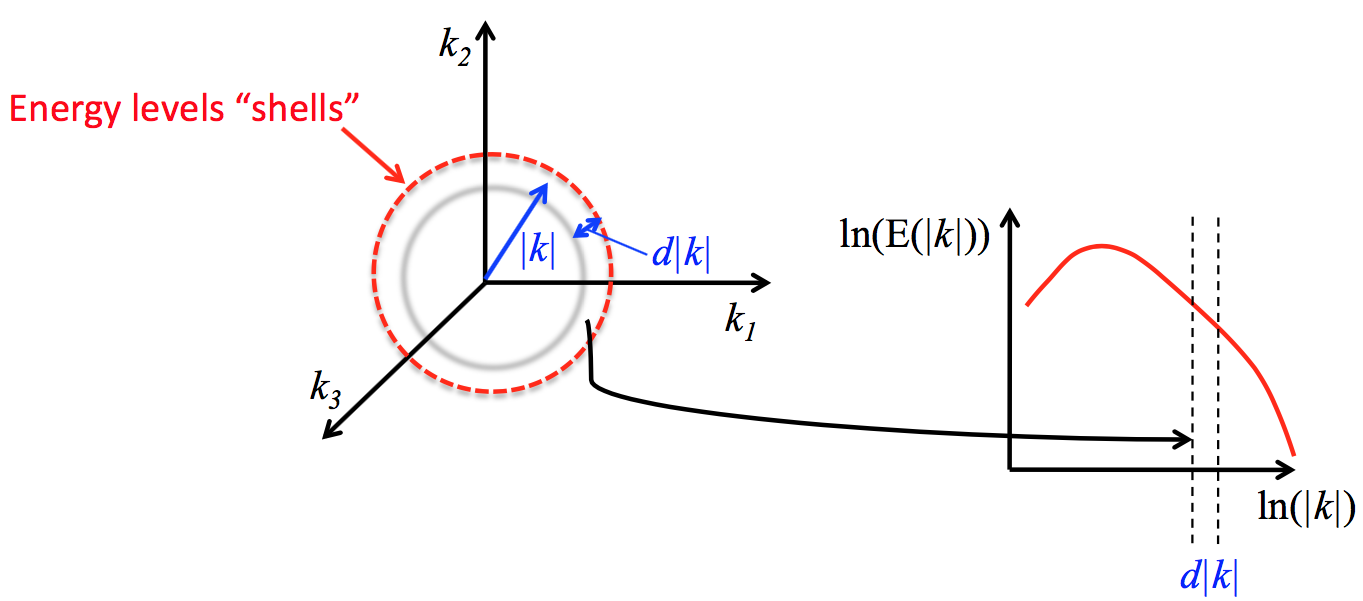
\includegraphics[width=\textwidth]{3dspectra1}
\end{figure}

\end{frame}

%------------------------------------------------

\begin{frame}{A quick chat about Homework \#2}

\begin{figure}
	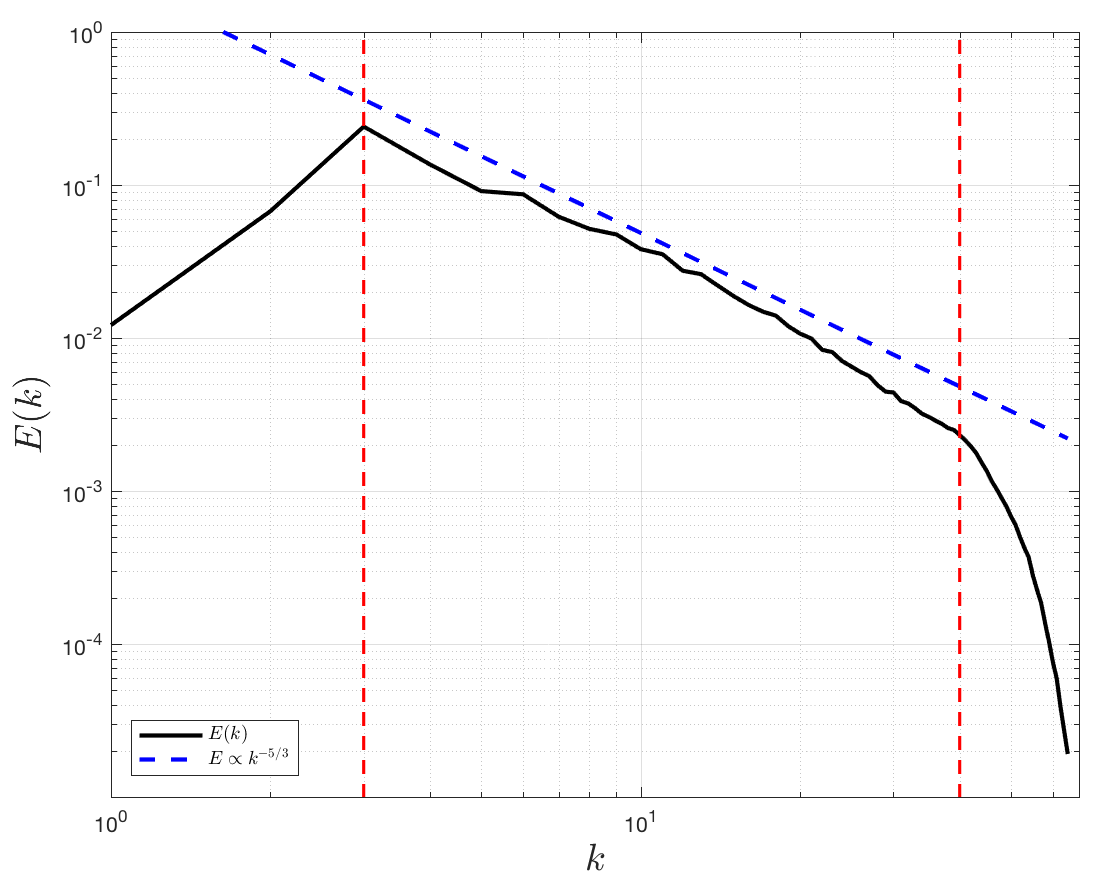
\includegraphics[width=0.9\textwidth]{3dspectra2}
\end{figure}

\end{frame}

%------------------------------------------------
\section{Classes of LES models for $\tau_{ij}$} %
%------------------------------------------------

\begin{frame}{Classes of LES models for $\tau_{ij}$}

\begin{itemize}
	\item Eddy-Viscosity Models
	\item Similarity Models
	\item Stochastic SGS Models
	\item Subgrid Velocity Reconstruction Models
	\item Dynamic Models
\end{itemize}

\end{frame}

%------------------------------------------------

\begin{frame}{Classes of LES models for $\tau_{ij}$}
\textbf{Eddy-Viscosity Models}
\begin{itemize}
	\item The largest and most commonly used class of SGS models.
	\item The general idea is that turbulent diffusion at SGSs (\textit{i.e.} how SGSs remove energy) is analogous to molecular diffusion. It is very similar in form to K-theory for Reynolds stresses.
\end{itemize}

\end{frame}

%------------------------------------------------

\begin{frame}{Classes of LES models for $\tau_{ij}$}
\textbf{Eddy-Viscosity Models}
\begin{itemize}
	\item The deviatoric part of $\tau_{ij}$ is modeled as
	$$\tau_{ij} - \frac{1}{3}\tau_{kk}\delta_{ij} = -2\nu_{T} \widetilde{S}_{ij}$$
	where $\nu_T$ is the SGS eddy-viscosity and 
	$$\widetilde{S}_{ij} = \frac{1}{2}\left( \frac{\partial \widetilde{u_i}}{\partial x_j} + \frac{\partial \widetilde{u_j}}{\partial x_i} \right)$$ is the strain rate tensor.
\end{itemize}
Within this class of models we have many different ways of determining $\nu_T$
\end{frame}


%------------------------------------------------

\begin{frame}{Classes of LES models for $\tau_{ij}$}
\textbf{Eddy-Viscosity Models}
\begin{itemize}
	\item Smagorinsky model (Smagorinsky 1963)
	\item ``Kolmolgorov'' eddy-viscosity model (Wong and Lilly 1994)
	\item Two-point closure models (based on Kraichan's (1974) spectral eddy-viscosity model and developed by Lesiour (see Lesiour et al. 2005)
	\item One-equation models that use the filtered KE equation (see Lecture 7 for the KE equation). An early application of the model is found in Deardorff (1980). An overview of the Deardorff model and possible modifications are given in Gibbs and Fedorovich (2016)
\end{itemize}

\end{frame}

%------------------------------------------------

\begin{frame}{Classes of LES models for $\tau_{ij}$}
\textbf{Similarity Models}
\begin{itemize}
	\item These models were first introduced by Bardina et al. (1980)
	\item Based on the idea that the most active SGSs are those close to the cutoff wavenumber (or scale)
	\item A subclass under this type of model is the nonlinear model
	\item These models are often paired with an eddy-viscosity model
\end{itemize}

\end{frame}

%------------------------------------------------

\begin{frame}{Classes of LES models for $\tau_{ij}$}
\textbf{Stochastic SGS Models}
\begin{itemize}
	\item In these models a random (stochastic) component is incorporated into the SGS model
	\item The nonlinear term is usually combined with an eddy-viscosity model as is done in similarity models (Mason and Thomson 1992)
\end{itemize}

\end{frame}

%------------------------------------------------

\begin{frame}{Classes of LES models for $\tau_{ij}$}
\textbf{Subgrid Velocity Reconstruction Models}
\begin{itemize}
	\item These models seek to approximate the SGS stress through a direct reconstruction of the SGS velocity or scalar fields
	\item Two examples are:
	\begin{itemize}
		\item fractal models (Scott and Meneveau 1999)
		\item linear-eddy and one-dimensional turbulence models (Kerstein 1988)
	\end{itemize}
\end{itemize}

\end{frame}

%------------------------------------------------

\begin{frame}{Classes of LES models for $\tau_{ij}$}
\textbf{Dynamic Models}
\begin{itemize}
	\item First developed by Germano (1991)
	\item Actually more of a procedure that can be applied to any base model
	\item One of the biggest and most influential ideas in LES SGS modeling
\end{itemize}

\end{frame}

%------------------------------------------------
\section{Testing SGS Models} %
%------------------------------------------------

\begin{frame}{Testing SGS Models - \textit{a posteriori}}
\textbf{\textit{a posteriori} testing}
\begin{itemize}
	\item Term can be credited to Piomelli et al. (1988)
	\item Run ``full'' simulations with a particular SGS model and compare the results (statistically) to DNS, experiments, or turbulence theory
	\item A ``complete'' test of the model (including dynamics and feedback)
	\item It has the disadvantage of including numerics and we can't gain insight into the physics of SGSs
\end{itemize}
\end{frame}

%------------------------------------------------

\begin{frame}{Testing SGS Models - \textit{a priori}}
\textbf{\textit{a priori} testing}
\begin{itemize}
	\item Use DNS or high resolution experimental data to test SGS models ``offline''
	\item \textbf{Goal}: directly compare $\tau_{ij}^{\Delta} (\vec{x}, t)$ with $\tau_{ij}^{\Delta, \text{M}} (\vec{x}, t)$
	\item How is this accomplished?
\end{itemize}

\end{frame}

%------------------------------------------------

\begin{frame}{Testing SGS Models - \textit{a priori}}
\textbf{\textit{a priori} testing}
\begin{itemize}
	\item Filter DNS (or experimental) data at $\Delta$ and compute the exact $\tau_{ij}^{\Delta} (\vec{x}, t)$ and other relevant parameters
	\item Use the filtered $u$,$v$, and $w$ to compute $\tau_{ij}^{\Delta, \text{M}} (\vec{x}, t)$ from the model (and stats) and compare with the above results. This can also be used to calculate unknown model coefficients
	\item Allows us to look specifically at how the model reproduces SGS properties and the physics associated with those properties
	\item Drawback -- it does not include dynamic feedback and numerics!
\end{itemize}

\end{frame}


%------------------------------------------------
\section{Eddy-Viscosity Models} %
%------------------------------------------------
\begin{frame}{Eddy-Viscosity Models}
\begin{itemize}
	\item See Guerts pg 225; Pope pg 587
	\item Eddy-viscosity models are of the form:
	\begin{align*}
		\text{momentum} \qquad \tau_{ij} &= -2\nu_{T} \widetilde{S}_{ij}\\
		\text{scalars} \qquad q_i &= -D_T \frac{\partial \widetilde{\theta}}{\partial x_i}
	\end{align*}
	where
	$$D_T = \frac{\nu_T}{\text{Pr}},$$
	\item $\widetilde{S}_{ij}$ is the filtered strain rate
	\item $\nu_T$ is eddy-viscosity
	\item $D_T$ is eddy-diffusivity
	\item Pr is the SGS Prandtl number 
\end{itemize}

\end{frame}

%------------------------------------------------
\begin{frame}{Eddy-Viscosity Models}
\begin{itemize}
	\item This is the LES equivalent to \nth{1}-order RANS closure (k-theory or gradient transport theory) and is an analogy to molecular viscosity (see Pope Ch. 10 for a review)
	\item Turbulent fluxes are assumed to be proportional to the local velocity or scalar gradients
	\item In LES, this is the assumption that stress is proportional to strain: $\tau_{ij} \sim \widetilde{S}_{ij}$
	\item The SGS eddy-viscosity $\nu_T$ must be parameterized   
\end{itemize}

\end{frame}

%------------------------------------------------
\begin{frame}{Eddy-Viscosity Models}
\begin{itemize}
	\item Dimensionally
	$$\nu_T = \left[ \frac{L^2}{T}\right]$$
	\item In almost all SGS eddy-viscosity models:
	$$\nu_T \sim U\ell$$
	\item Different models use different $U$ and $\ell$
\end{itemize}

\end{frame}

%------------------------------------------------
\begin{frame}{Eddy-Viscosity Models}
\begin{itemize}
	\item Recall the filtered N-S equations
	$$\frac{\partial \tilde u_i}{\partial t} + \frac{\partial (\tilde u_i \tilde u_j)}{\partial x_j} = - \frac{\partial \tilde p}{\partial x_j} + \underbrace{\frac{1}{\text{Re}} \frac{\partial^2 \tilde u_i}{\partial x_j^{2}}}_{1} -\underbrace{\frac{\partial \tau_{ij}}{\partial x_j}}_{2}+ F_i$$
	\item Let's focus on the viscous and subgrid stress terms 
\end{itemize}

\end{frame}

%------------------------------------------------
\begin{frame}{Eddy-Viscosity Models}
\begin{itemize}
\item Viscous term
	\begin{align*}
		 \frac{1}{\text{Re}} \frac{\partial^2 \tilde u_i}{\partial x_j^{2}} &= \frac{1}{\text{Re}}\frac{\partial}{\partial x_j} \left(\frac{\partial \tilde u_i}{\partial x_j}\right) = \frac{1}{\text{Re}} \frac{\partial}{\partial x_j} \left(\frac{\partial \tilde u_i}{\partial x_j} + \frac{\partial \tilde u_j}{\partial x_i} - \frac{\partial \tilde u_j}{\partial x_i}\right)\\
		 &= \frac{2}{\text{Re}} \frac{\partial \widetilde{S}_{ij}}{\partial x_j} -  \frac{1}{\text{Re}} \frac{\partial}{\partial x_j} \left( \frac{\partial \tilde u_j}{\partial x_i}\right)\\
		 &= \frac{2}{\text{Re}} \frac{\partial \widetilde{S}_{ij}}{\partial x_j} -  \frac{1}{\text{Re}} \frac{\partial}{\partial x_i} \cancelto{0}{\left(\frac{\partial \tilde u_j}{\partial x_j}\right)}\\
		 &= \frac{2}{\text{Re}} \frac{\partial \widetilde{S}_{ij}}{\partial x_j}
	\end{align*}
\end{itemize}
\end{frame}

%------------------------------------------------
\begin{frame}{Eddy-Viscosity Models}
\begin{itemize}
\item SGS stress term
	\begin{align*}
		 \frac{\partial \tau_{ij}}{\partial x_j} &= -\frac{\partial (2 \nu_T \widetilde{S}_{ij})}{\partial x_j}\\
		 &= -2\frac{\partial (\nu_T \widetilde{S}_{ij})}{\partial x_j}
	\end{align*}
\end{itemize}
\end{frame}


%------------------------------------------------
\begin{frame}{Eddy-Viscosity Models}
\begin{itemize}
\item Combining the terms yields a new (approximate) viscous term
	$$\frac{1}{\text{Re}} \frac{\partial^2 \tilde u_i}{\partial x_j^{2}} -\frac{\partial \tau_{ij}}{\partial x_j} = \boxed{2\frac{\partial}{\partial x_j}\left[\left(\nu_T + \frac{1}{\text{Re}}\right)\widetilde{S}_{ij}\right]}$$
	\item If we were to write this in dimensional form:
	$$\boxed{2\frac{\partial}{\partial x_j}\left[\left(\nu_T + \nu\right)\widetilde{S}_{ij}\right]}$$
	Thus, we can interpret the eddy-viscosity as adding to the molecular viscosity.
\end{itemize}
\end{frame}

%------------------------------------------------
\begin{frame}{Eddy-Viscosity Models}
\begin{itemize}
	\item The eddy-viscosity extracts energy from the resolved scales in the simulation
	\item It mimics the average energy transfer in the turbulent cascade
	\item E-V model only transfer energy from resolved to subgrid -- meaning the models only represent the statistically-averaged flow of energy and not the combined instantaneous forward scatter and backscatter
\end{itemize}

\end{frame}

%------------------------------------------------
\begin{frame}{Eddy-Viscosity Models}
$$2\frac{\partial}{\partial x_j}\left[\left(\nu_T + \nu\right)\widetilde{S}_{ij}\right]$$
\newline\newline
\textbf{What does the model do?}
\begin{itemize}
	\item We can see it effectively lowers the Reynolds number of the flow
	\item It provides all of the energy dissipation for high Re flows (when 1/Re$\Rightarrow$0).
\end{itemize}
\end{frame}

%------------------------------------------------

\begin{frame}{Eddy-Viscosity Models}
\textbf{Most LES models use a nonlinear eddy viscosity. What happens if we use a constant?} 
\begin{itemize}
	\item We effectively run the simulation at a different (lower) Re
	\item This has implications for DNS -- if we try to use DNS at a lower Re to examine phenomena that happens at a higher Re, we can make the analogy between our DNS and an LES with a SGS model that doesn't properly reproduce the flow physics
\end{itemize}
\end{frame}


%------------------------------------------------

\end{document}

